%%-----------Chapter 4------------------------------------------
\chapter{Newton's Three Laws of Motion}

Before stating any law, it is worth asking a simple question. What does it take for something
to keep moving? If you roll a ball across the floor, what eventually stops it?

The instinctive answer, and the one given by Aristotle for well over a thousand years, is
that motion requires a continuous sustaining force. Remove the force and the motion should
stop. This view matches what we see every day: carts roll to a halt, thrown balls fall back,
skidding cars come to rest. The trouble is that it is wrong. What actually stops a rolling
ball is friction, not the absence of some hidden push. In the absence of friction (or any
other opposing force), the ball would continue rolling forever. This is the content of
Newton's first law, but it took from Aristotle to Galileo to articulate it clearly, and from
Galileo to Newton to place it in its proper setting.

\section{The First Law (the Law of Inertia)}

\begin{keybox}[The First Law]
In the absence of a net external force, a body at rest remains at rest, and a body in
motion continues to move at constant velocity.
\end{keybox}

The tendency of a body to continue in its initial state of motion is called its \textbf{inertia}.
Accordingly, the First Law is often called the \textbf{Law of Inertia}. Written as an equation:
\begin{equation}
  \sum\vec{F} = 0 \iff \vec{a} = 0.
\end{equation}
This is less a statement about motion than a statement about force: force is not what
\emph{maintains} motion, but what \emph{changes} it. A body travelling at constant velocity is no
more mysterious than a body at rest --- both are states of zero acceleration, and both require
zero net force.

There is a subtlety in the first law that is easy to miss. The first law holds only in an
\textbf{inertial frame} --- a frame that is not itself accelerating. The car that brakes
suddenly is not such a frame; viewed from the ground, the ball on the dashboard is simply
continuing in a straight line at constant velocity while the car decelerates around it.

Is the Earth an inertial frame? Strictly speaking, no. But quantitatively: the Earth's
orbital radius is $R\approx1.5\times10^{11}\,\text{m}$ and its orbital period is
$T\approx3.15\times10^7\,\text{s}$, giving an orbital speed
\begin{equation}
  v = \frac{2\pi R}{T} \approx 2.99\times10^4\;\text{m/s}
\end{equation}
and a centripetal acceleration
\begin{equation}
  a = \frac{v^2}{R} \approx 6\times10^{-3}\;\text{m/s}^2.
\end{equation}
Compared to $g=9.8\,\text{m/s}^2$, this is smaller by a factor of roughly 1600. Newton's
first law therefore holds as an extraordinarily good approximation, and we will use it as if
it were exact.


\section{The Second Law}

\begin{keybox}[The Second Law]
For any particle of mass $m$, the net force $\vec{F}$ on the particle is always equal to the
mass $m$ times the particle's acceleration:
\begin{equation}
  \vec{F} = m\vec{a}.
\end{equation}
\end{keybox}

Three points are worth emphasising:
\begin{enumerate}
  \item $\vec{F}$ is the \emph{net} force --- the vector sum of \emph{all} forces acting on the body.
  \item The equation is a \emph{vector equation}: it must hold component by component, and in
        particular the acceleration vector always points in the same direction as the net force.
  \item Despite appearances, this is \emph{not} a definition of force. Force has an independent
        physical meaning, and the second law is the (enormously successful) empirical claim that
        force and acceleration are proportional, with the constant of proportionality being the
        body's mass.
\end{enumerate}

As a simple application, consider two blocks of mass $m_1$ and $m_2$ connected by a light
inextensible rope on a frictionless horizontal surface, with a horizontal force $F$ applied to
$m_2$ pulling the pair along. Treating the pair as a single system of mass $M=m_1+m_2$, the
acceleration is
\begin{equation}
  a = \frac{F}{m_1+m_2}.
\end{equation}
To find the tension in the rope we isolate $m_1$. The only horizontal force on $m_1$ is the
tension $T$, so
\begin{equation}
  T = m_1\,a = \frac{m_1 F}{m_1+m_2}.
\end{equation}
This example illustrates a general strategy. When several bodies are connected, it often pays
to treat them first as a single system (to find the common acceleration), and then isolate
each body in turn (to find internal forces like tension).

\begin{figure}[H]
  \centering
  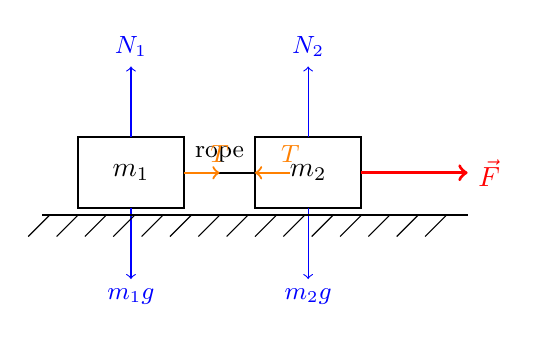
\begin{tikzpicture}[scale=0.9]
    % Two blocks
    \draw[thick] (0,0) rectangle (1.5,1) node[midway]{$m_1$};
    \draw[thick] (2.5,0) rectangle (4,1) node[midway]{$m_2$};
    % Rope
    \draw[thick] (1.5,0.5) -- (2.5,0.5) node[above,midway]{\small rope};
    % Applied force
    \draw[->,very thick,red] (4,0.5) -- (5.5,0.5) node[right]{$\vec{F}$};
    % Normal forces
    \draw[->,blue] (0.75,1) -- (0.75,2) node[above]{\small $N_1$};
    \draw[->,blue] (3.25,1) -- (3.25,2) node[above]{\small $N_2$};
    % Weights
    \draw[->,blue] (0.75,0) -- (0.75,-1) node[below]{\small $m_1 g$};
    \draw[->,blue] (3.25,0) -- (3.25,-1) node[below]{\small $m_2 g$};
    % Tension arrows on rope
    \draw[->,thick,orange] (1.5,0.5) -- (2.0,0.5) node[above]{\small $T$};
    \draw[<-,thick,orange] (2.5,0.5) -- (3.0,0.5) node[above]{\small $T$};
    % Ground
    \draw[thick] (-0.5,-0.1) -- (5.5,-0.1);
    \foreach \x in {-0.4,-0.0,0.4,0.8,...,5.4}
      \draw[thin] (\x,-0.1) -- (\x-0.3,-0.4);
  \end{tikzpicture}
  \caption{Two blocks connected by a light rope on a frictionless surface. Horizontally,
  $m_1$ is pulled only by the tension $T$, while $m_2$ is pulled forward by $F$ and backward by $T$.}
\end{figure}


\section{The Third Law}

\begin{keybox}[The Third Law]
If object 1 exerts a force $\vec{F}_{21}$ on object 2, then object 2 will exert a reaction
force $\vec{F}_{12}$ on object 1 given by
\begin{equation}
  \vec{F}_{12} = -\vec{F}_{21}.
\end{equation}
\end{keybox}

The crucial point, and the one most often misunderstood, is that these two forces act on
\textbf{different bodies}. They therefore never cancel each other.

Let us apply this to a familiar situation. You drop an apple. The Earth pulls the apple
downward with gravitational force $F=mg$. By the third law, the apple must pull the Earth
upward with an equal force. The apple's acceleration is
\begin{equation}
  a_\text{apple} = \frac{F}{m_\text{apple}} = g \approx 9.8\;\text{m/s}^2.
\end{equation}
The Earth's acceleration is
\begin{equation}
  a_\text{Earth} = \frac{F}{M_\text{Earth}} = \frac{mg}{M_\text{Earth}}.
\end{equation}
Taking a 100\,g apple and $M_\text{Earth}\approx5.97\times10^{24}\,\text{kg}$:
\begin{equation}
  a_\text{Earth} \approx 1.6\times10^{-25}\;\text{m/s}^2.
\end{equation}
Over the roughly half-second duration of the apple's fall, the Earth moves toward the apple
by a distance far smaller than the diameter of a proton.

The principle scales up. The third law is also at the root of the \textbf{horse-cart paradox}.
A horse pulls a cart forward. By the third law, the cart pulls the horse backward with an
equal force. So how does anything ever move? The resolution: the forward pull on the cart
and the backward pull on the horse act on \emph{different bodies}. To understand the horse's
motion we must look at all forces on the horse, which includes not only the backward pull
from the cart but also the forward friction from the ground on its hooves. Both the horse
and cart accelerate together. No paradox, only careful bookkeeping.


\section*{Class Exercise: The Atwood Machine}
\addcontentsline{toc}{section}{Class Exercise: The Atwood Machine}

Two blocks are connected by a light, inextensible string passing over a small frictionless
pulley fixed to the ceiling. Block 1 has mass $m_1=6\,\text{kg}$ and Block 2 has mass
$m_2=4\,\text{kg}$. The system is released from rest. Take $g=10\,\text{m/s}^2$.

\begin{figure}[H]
  \centering
  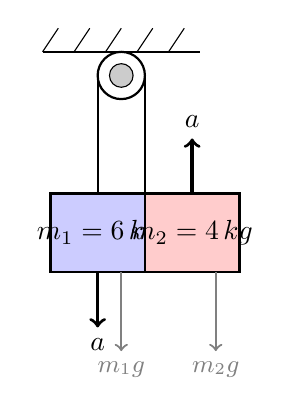
\begin{tikzpicture}
    % Pulley
    \draw[thick] (0,0) circle (0.3);
    \draw[fill=gray!40] (0,0) circle (0.15);
    % Ceiling
    \draw[thick] (-1,0.3) -- (1,0.3);
    \foreach \x in {-1,-0.6,...,0.9}
      \draw[thin] (\x,0.3) -- (\x+0.2,0.6);
    % Strings
    \draw[thick] (-0.3,0) -- (-0.3,-1.5);
    \draw[thick] (0.3,0)  -- (0.3,-1.5);
    % Blocks
    \draw[thick,fill=blue!20] (-0.9,-1.5) rectangle (0.3,-2.5) node[midway]{$m_1=6\,\text{kg}$};
    \draw[thick,fill=red!20]  (0.3,-1.5)  rectangle (1.5,-2.5) node[midway]{$m_2=4\,\text{kg}$};
    % Acceleration arrows
    \draw[->,very thick] (-0.3,-2.5) -- (-0.3,-3.2) node[below]{$a$};
    \draw[->,very thick] (0.9,-1.5) -- (0.9,-0.8) node[above]{$a$};
    % Weight labels
    \draw[->,thick,gray] (0,-2.5) -- (0,-3.5) node[below]{\small $m_1 g$};
    \draw[->,thick,gray] (1.2,-2.5) -- (1.2,-3.5) node[below]{\small $m_2 g$};
  \end{tikzpicture}
  \caption{The Atwood Machine. Block 1 ($m_1=6\,\text{kg}$) descends while Block 2 ($m_2=4\,\text{kg}$) ascends.}
\end{figure}

\begin{enumerate}[label=(\alph*)]
  \item Draw a free body diagram for each block and write down Newton's second law for each.
  \item Hence find the acceleration $a$ of the system and the tension $T$ in the string.
  \item What is the tension in the string if both masses were equal? Comment on your answer physically.
\end{enumerate}




